\section{Memorymanagement}

Es gibt verschiedene Gründe warum nicht immer gleich viel Speicher verwendet wird z.B. da nicht unbegrenzt vorhanden ist.
Speicher wird nur dann verwendet, wenn er wirklich gebraucht wird. 
Das Memorymanagement muss aktiv beachtet werden.
Es wird zwischen automatischen und manuellen Speichermanagement unterschieden. 

\subsection{Automatisch}

Automatisches Speichermanagement wird anhand der Lebenszeit einer Variable festgestellt und während dem Programmieren bereits festgelegt. 
Der Speicher liegt auf dem sogenannten \textbf{Stapel / Stack}.\\
Wird eine Funktion aufgerufen, werden die benötigten Variablen auf dem Stack definiert. 
Ebenso wird eine Returnadresse zur Funktion, die die Funktion aufgerufen hat abgelegt.
Wie die Daten angeordnet werden, ist Architektur-abhängig.
Wird die Funktion wieder verlassen, werden die Variablen vom Stack wieder entfernt und zur aufrufenden Funktion zurückgesprungen.  

\subsection{Manuell/dynamisch}

Man kann auch manuell Speicher anfordern. 
Zum Beispiel, falls zur Compilezeit nicht bekannt ist, wie viel Speicher gebraucht wird.
Dieser Speicher ist auf dem sogenannten \textbf{Haufen / Heap}.\\
Der Heap ist ein Speicherbereich, der vom Betriebssystem bereitgestellt und verwaltet wird.\\
Zur Laufzeit wird Speicher dynamisch angefordert. 
Dieser bleibt so lange belegt bis dieser Manuell wieder freigegeben wird.\\
Es kann aber auch sein, falls der Speicher stark fragmentiert ist, das kein Speicher bereitgestellt werden kann. 
Generell ist bei sehr vollem Speicher das Arbeiten erschwert.

\subsubsection{Speicherlecks}

Falls ein Programm unkontrolliert Speicher aufnimmt oder den ihm zur Verfügung gestellte nicht wieder freigibt, spricht man von einem Speicherleck. 
Diese sind zu verhindern da diese zu einer Systemüberlastung und Abstürzen führen.


\subsection{Speichermanagement funktionen}

Es gibt einige Funktionen für Speichermanagement. In C und C++ sind diese leicht verschieden. 
Generell geben diese einen Pointer zurück, welcher auf freien Speicher zeigt. 
\textbf{Diese müssen immer auf einen Nullpointer geprüft werden, da keine Garantie vorhanden ist, ob überhaupt Speicher vorhanden ist!}
Generell sollte mit solchen Pointer immer misstrauisch gearbeitet werden und nach Abschluss immer wieder freigegeben werden.

\subsubsection{C: malloc( ) calloc( ), free( ) (Funktionen)}

\textbf{malloc()} gibt einen Voidpointer(pointercasting nicht vergessen) zurück welche auf eine angeforderte Grösse an Bytes Speicher zeigt. 
Der Speicher ist \textbf{nicht} initialisiert
\textbf{calloc()} macht dasselbe, initialisiert aber den Speicher auf 0.\\
\textbf{free()} gibt den Speicherbereich wieder frei.

\lstinputlisting{code/mem_mngmt_c.c}

Falls kein Speicher allokiert werden kann, wird ein NULL-pointer zurückgegeben.

\subsubsection{C++: new, delete, new[ ], delete[ ] (Operatoren)}

Der \textbf{new}-Operator erstellt ein Pointer welcher auf die mitgegebene Grösse zeigt.
\textbf{new[ ]} macht dasselbe, ausser das dieser ein Array zurückgibt.

\textbf{delete} / \textbf{delete[ ]} gibt den Speicher wieder frei. 
Dieser kann auch auf den Nullpointer ausgeführt werden. 
Dieser ist \say{Delete} egal.

\lstinputlisting{code/mem_mngmt_cpp.cpp}

\nextcol

\subsection{Speicheraufbau}

Der Speicheraufbau bildlich dargestellt sieht ungefähr so aus:

\begin{center}
    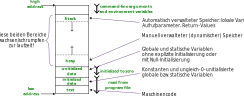
\includegraphics[width=\columnwidth]{pictures/memorylayout.png}  
\end{center}

Je nach Architektur kann es auch sein, dass die hohen und tiefen Adressen anders herum sind.

\subsection{Referenzen}

Referenzen sind die modernere / eingeschränkte Version von Pointer. 
Wenn möglich sollte immer mit Referenzen gearbeitet werden, dies ist aber nicht immer möglich.\\

Referenzen...
\begin{itemize}[itemsep=1pt, parsep=0pt]
    \item wirken wie ein Alias-Name einer Variablen
    \item werden wie normale Variablen verwendet
    \item sind niemals uninitialisiert
    \item haben niemals den Wert nullptr
    \item brauchen nicht immer Speicher (Implementations abhängig)
\end{itemize}

Generell helfen Referenzen weniger Fehler in der Programmierung zu machen und weniger Risiken zu haben. 
Pointer werden allerdings weiter für sehr hardwarenahe Programmierung gebraucht. 
\textbf{sizeof()} liefert die Grösse des Typs, auf der die Referenz zeigt.\\
Beispiel:

\lstinputlisting{code/referenz.cpp}

\subsection{Speicherplatzbedarf von Objekten}

Eine Unterklasse braucht immer mindestens so viel speicher wie eine Oberklasse.

\subsubsection{Zuweisungen}

Zuweisungen von Oberklasse zu Unterklasse sind in der regel möglich da alle geerbten Attribute ja vorhanden sind. 
Umgekehrt geht das allerdings nicht, da der Speicher dafür nicht initialisiert ist.

\subsection{Type Casting}

\begin{center}
    \rotatebox{90}{%            
    \resizebox{1.7 \columnwidth}{!}{%
    \begin{tabular}{|c|l|l|l|}
        \hline
        {\color{blue} Cast:} &
          \multicolumn{1}{c|}{{\color{blue} Anwendungsbereiche}} &
          \multicolumn{1}{c|}{{\color{blue} Wissenswertes}} &
          \multicolumn{1}{c|}{{\color{blue} Beispiele}} \\ \hline
        {\color{blue} \begin{tabular}[c]{@{}c@{}}implizit: \\ kein Cast\end{tabular}} &
          \begin{tabular}[c]{@{}l@{}}• Numerische Typen u. bool\\ (ggf. mit Warnung, falls Wertebereich\\ möglicherweise nicht ausreicht)\\ • Objektinstanzen einer Unterklasse in\\ einer Variablen vom Typ der\\ Oberklasse speichern (Upcast).\\ • Pointertypen, deren Umkonvertierung\\ «ungefährlich» ist – die genauen\\ Regeln sind ziemlich kompliziert.\end{tabular} &
           &
          \begin{tabular}[c]{@{}l@{}}1. {\color{codeGreen}signed char} a = 1;\\ {\color{codeGreen}int} b = a;\\ \\ 2. {\color{codeGreen}int} a = 1;\\ {\color{codeGreen}char} b = a; {\color{blue}// ggf. mit Warnung}\\ \\ 3. Bird b;\\ Animal a = b; {\color{blue}// Upcast: a ist ein Animal}\end{tabular} \\ \hline
        {\color{blue} static} &
          \begin{tabular}[c]{@{}l@{}}• Alles, was implizit möglich ist,\\ unterdrückt dabei etwaige Warnungen.\\ • Pointer- und Referenz-Typen auf\\ Instanzen von Ober- und\\ Unterklassen in beide Richtungen\\ umwandeln: Upcast und\\ Downcast (\textbf{ohne Typprüfung} zur\\ Laufzeit, Auswertung\\ ausschliesslich zur \textbf{Compilezeit})\end{tabular} &
           &
          \begin{tabular}[c]{@{}l@{}}1. {\color{codeGreen}int} a = 1;\\ {\color{codeGreen}char} b = {\color{codeGreen}static\_cast}\textless{}{\color{codeGreen}char}\textgreater{}(a);\\ 2. Bird* b = {\color{codeGreen}new} Bird;\\ Animal* a = b; {\color{blue}// geht implizit!}\\ Bird* c = {\color{codeGreen}static\_cast}\textless{}Bird*\textgreater{}(a);\\ {\color{blue}/* Braucht einen down-Cast} , \\ {\color{codeGreen}weil nicht jedes Animal ein Bird ist!*/}\end{tabular} \\ \hline
        {\color{blue} dynamic} &
          \begin{tabular}[c]{@{}l@{}}• Pointer- und ReferenzTypen auf \\ Instanzen von\\ \textbf{polymorphen} Ober- und\\ Unterklassen in beide\\ Richtungen umwandeln:\\ Upcast und Downcast (\textbf{mit}\\ Typprüfung per RTTI zur\\ Laufzeit)\end{tabular} &
          \begin{tabular}[c]{@{}l@{}}Unterstützt ausserdem einen\\ Upcast für Pointer- und\\ Referenztypen auf nichtpolymorphe Klassen\\ (normalerweise machen wir dies aber \\ implizit oder verwenden einen static\_cast!)\\ Falls der dynamic\_cast \textbf{fehlschlägt}, liefert \\ er bei Pointer-Typen den Wert\\ \textbf{nullptr}, bei Referenzen wird\\ eine \textbf{std::bad\_cast-Exception} geworfen\end{tabular} &
          \begin{tabular}[c]{@{}l@{}}Animal* a = {\color{codeGreen}new} Ant;\\ Bird* b = {\color{codeGreen}dynamic\_cast}\textless{}Bird*\textgreater{}(a);\\ {\color{blue}/* Der Dynamic Cast wird}\\ {\color{blue}immer zur Laufzeit ausgewertet.  dh:}\\ {\color{blue}b ==nullptr */}\end{tabular} \\ \hline
        {\color{blue} const} &
          \begin{tabular}[c]{@{}l@{}}verändert die \say{constness} und/oder\\ \say{volatile-ness} des\\ Ziels eines Pointeroder ReferenzTyps.\end{tabular} &
           &
          \begin{tabular}[c]{@{}l@{}}{\color{codeGreen}const int} val = 10; \\ {\color{codeGreen}const int} *ptr = \&val; \\ {\color{codeGreen}int} *ptr1 = {\color{codeGreen}const\_cast} \textless{}{\color{codeGreen}int} *\textgreater{}(ptr);\end{tabular} \\ \hline
        {\color{blue} reinterpret} &
          \begin{tabular}[c]{@{}l@{}}• Konvertiert zwischen beliebigen Pointer-Typen \\ sowie zwischen beliebigen Pointer und int-Typen \\\textbf{ohne Typprüfung}.\\ • Kann auch mit Referenz-Typen\\ umgehen.\end{tabular} &
          \begin{tabular}[c]{@{}l@{}}Achtung: erzeugt\\ plattformspezifisches Verhalten\end{tabular} &
          \begin{tabular}[c]{@{}l@{}}Animal* a = {\color{codeGreen}new} Ant;\\ \\ {\color{codeGreen}uint8\_t}* b =\\ {\color{codeGreen}reinterpret\_cast}\textless{}{\color{codeGreen}uint8\_t}*\textgreater{}(a);\end{tabular} \\ \hline
        \end{tabular}%
    }
    }          
\end{center}

Die C Syntax für Casting sollte nicht mehr verwendet werden da meistens nicht optimales verhalten. 

\nextcol

\subsection{Templates}

Templates erlauben es Typen-unabhängigen Code zu schreiben. 
Eine Funktion wird mit einem \textbf{Platzhalter-typ} geschrieben. 
Bei der Verwendung wird ein oder mehrere zu verwendende Typen mitgegeben (es ist auch möglich Konstanten mitzugeben). 
Es sind Klassen und Funktionstemplates möglich. 
Templates werden immer zur \textbf{Compilezeit} ausgewertet. 
Templates brauchen eine Deklaration, Definition und Instanziierungsparameter. 
Sie werden ausschliesslich in einem H-File deklariert.\\
Achtung! Templates werden für jeden \textbf{unterschiedlichen} Typen der Instanziiert wird angelegt. 
Das kann zu hohem Speicherbedarf führen.

\subsubsection{Implementation}

Eine Funktion / Klasse kann als Template definiert werden indem \say{template $<$typename1 T1, typename2 T2, ...$>$ } (mit\say{$<>$}) vor die Funktion / Klasse geschrieben wird. 
Die Typendefinitionen sind dann durch das T zu ersetzten. 

\lstinputlisting{code/templatesswap.cpp}

\subsubsection{Syntax}

\lstinputlisting{code/templatesyntax.cpp}

\subsubsection{Instanziierung}

\textbf{Klassentemplates} (\say{$<>$} braucht es) :\\
\say{Templatenamename}$<$type1, type2, ...$>$ \say{Instanzname}\\

\textbf{Funktionstemplates} (\say{$<>$} braucht es):\\
\say{Templatenamename}$<$type1, type2, ...$>$(param1, ...);\\

Falls bei der Instanziierung des Funktionstemplates der Typ bereits klar ist, können diese weggelassen werden. 

\nextcol

\section{Exceptions}

Exceptions werden zur Behandlung von Fehlern verwendet. 
Eine Exception ist eine Instanz eines beliebigen Datentyps, welche Fehlerinformation transportiert. 
Eine Exception wird bei Fehlerauftritt \say{geworfen} (throw), und zur Behandlung \say{gefangen} (catch).


\lstinputlisting{code/exceptionGenerellSyntax.cpp}

Diese Syntax ist so in der Praxis wenig aufzufinden da das Fehler werfen meist in einer Unterfunktion gemacht wird. 
Eine geworfene Exception wird dann mit code um die Instanziierung gehandhabt. 
Dies erlaubt es Fehler von Unterfunktionen je nach Situation anders zu handhaben:

\lstinputlisting{code/throwCatchV2.cpp}

Cout:

\begin{itemize}[itemsep=1pt, parsep=0pt]
    \item Entering foo()
    \item Not optimal but ok, Division by zero!
    \item Continue Programm
    \item Entering foo()
    \item Critical error: Division by zero!
    \item Program terminating
\end{itemize}

\subsection{Mehrere Catch Blöcke}

Unterschiedliche Exceptions können mit mehreren seriellen Catch Blöcken erreicht werden. 
Wenn der letzte Catch block mit \say{...} aufgerufen wird, werden alle Typen Exceptions gehandelt. 

\nextcol

\lstinputlisting{code/catchcatcher.cpp}

\subsection{Fehlender catch block}

Falls kein Passender catch Block gefunden werden kann wird die Funktion std::terminate() aufgerufen. 
Diese ruft den registrierten \textbf{std::terminate\_handler} (Funktionspointer). 
Defaultmässig ist \textbf{std::abort()} hinterlegt welche das Programm beendet ohne Destruktoren zu rufen (crash).
Falls dieses Verhalten angepasst werden soll, kann man das mit \say{set\_terminate(std::terminate\_handler f)}.

\subsection{leerer Catch block}

\colorbox{red!50}{\textit{straight to hell}}

\subsection{noexcept}

Um zu signalisieren, ob eine Funktion eine Exception auslösen kann oder nicht, kann der specifier \say{\textbf{noexept}} verwendet werden. 
Dafür ist aber \textbf{der Entwickler zuständig}. 
Der Compiler kann \textbf{nicht} prüfen, ob die Funktion tatsächlich eine Exception wirft oder nicht. 

\subsection{$<$stdexcept$>$}

\textbf{stdexcept} ist dazu da um einen einfachen Austausch von Fehlerinformationen vorzunehmen. 
Dafür sind diverse standardisierte Fehlertypen als Klassen definiert. Z.b.:\\
\begin{tabular}{ccc} \textbf{std::logic\_error} & \textbf{std::out\_of\_range} & \textbf{std::overflow\_error} \end{tabular}
Für Details siehe :\\
\url{https://en.cppreference.com/w/cpp/header/stdexcept}
\section{std:vector}
std:vector ist ein Klassentemplate welches die Kapazität selbständig bei Bedarf erweitert.
\lstinputlisting{code/vector.cpp}